	\newpage	
\center{\section{Постановка задачи}}


\flushleft{Реализовать алгоритмы сортировки массивов, найти сложность этих алгоритмов и провести временные эксперименты}


%%%%%%%%%%%%%%%%%%%%%%%%%%%%%%

\newpage
\center{\section{Блок-схемы}}


% 2 изображения в 1 строке
\begin{figure}[h!]	
	\begin{minipage}[h]{0.49\linewidth}
		\center{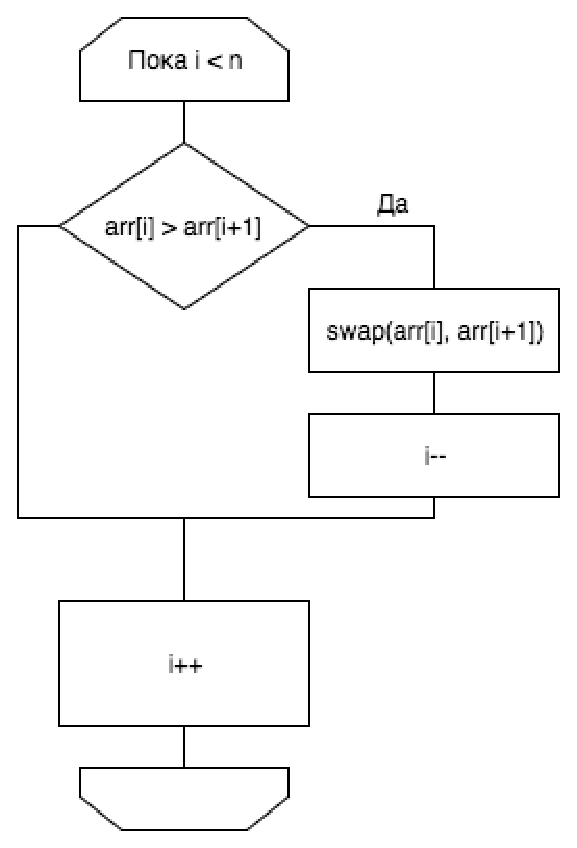
\includegraphics[width=\linewidth]{gnome}}
		\caption{Блок-схема Гномьего алгоритма}
	\end{minipage}
	\hfill
	\begin{minipage}[h]{0.49\linewidth}
		\center{\includegraphics[width=\linewidth]{bubble}}
		\caption{Блок-схема алгоритма Пузырька}
	\end{minipage}
\end{figure}

%\newpage

\begin{figure}
	\begin{minipage}{\linewidth}
		\center{\includegraphics[width=0.45\linewidth]{shaker}}
		\caption{Блок-схема алгоритма Шейкера}
	\end{minipage}
\end{figure}



%%%%%%%%%%%%%%%%%%%%%%%%%%%%%%

\newpage
\center{\section{Листинг}}

\textbf{\textsc{main.cpp:}}
\lstset{breaklines=true, numbers=left,
	keywordstyle=\color{blue}, commentstyle=\color{red}}
\lstinputlisting[language=c++]{../source/main.cpp}

\vspace{\baselineskip}

\textbf{\textsc{sorts.cpp:}}
\lstset{breaklines=true, numbers=left}
\lstinputlisting[language=c++]{../source/sorts.cpp}


%%%%%%%%%%%%%%%%%%%%%%%%%%%%%%	


\newpage
\center{\section{Временные  эксперименты  }}

\flushleft
Измерения производились для вещественных массивов

\begin{center}
	\begin{tabular}{|c|c|c|c|}
		\hline
		Размер массива & Отсортированный & Отсортированный в обратном порядке & Cлучайный\\
		
		\hline
		100 &0,1030 & 0,9690 & 0,2486 \\	
		
		\hline
		200 & 0,3601 & 0,0993 & 0,8915 \\	
		
		\hline
		300 & 0,8249 & 0,0132 & 1,9465 \\	
		
		\hline
		400 & 1,4108 & 0,0056 & 3,2779 \\	
		
		\hline
		500 & 2,3467 & 0,0065 & 5,0020 \\	
		
		\hline 
		600 & 3,3259 & 0,0075 & 7,2402 \\	
		
		\hline
		700 & 4,6154 & 0,0094 & 9,6110 \\	
		
		\hline
		800 & 5,9703 & 0,0103 & 12,7577 \\	
		
		\hline
		900 & 7,6857 & 0,0111 & 15,8312 \\	
		
		\hline
		1000 & 9,6741 & 0,0123 & 17,2874\\	
		
		\hline
		
	\end{tabular}
\end{center}	
\center{\textsc{Замеры времени в мс (среднее из 10 замеров) для Гномьей сортировки\\}}

\begin{center}
	\begin{tabular}{|c|c|c|c|}
		\hline
		Размер массива & Отсортированный & Отсортированный в обратном порядке & Случайный\\
		
		\hline
		100 & 0,0340 & 0,0637 & 0,0893 \\	
		
		\hline
		200 & 0,1094 & 0,2910 & 0,2853 \\	
		
		\hline
		300 & 0,4105 & 0,6484 & 0,6150 \\	
		
		\hline
		400 & 0,5323 & 0,9075 & 1,1760 \\	
		
		\hline
		500 & 0,7580 & 1,3810 & 1,8694 \\	
		
		\hline 
		600 & 1,0835 & 2,5466 & 2,6311 \\	
		
		\hline
		700 & 1,5378 & 3,4827 & 4,1932 \\	
		
		\hline
		800 & 2,1313 & 4,8444 & 5,0369 \\	
		
		\hline
		900 & 2,4246 & 5,4381 & 6,1783 \\	
		
		\hline
		1000 & 3,7684 & 6,0300 & 7,3179 \\	
		
		\hline
		
		
	\end{tabular}
\end{center}	
\center{\textsc{Замеры времени в мс (среднее из 10 замеров) для Пузырьковой сортировки\\}}

\begin{center}
	\begin{tabular}{|c|c|c|c|}
		\hline
		Размер массива & Отсортированный & Отсортированный в обратном порядке & Случайный\\
		
		\hline
		100 & 0,0014 & 0,0551 & 0,0941 \\
		
		\hline
		200 & 0,0024 & 0,1715 & 0,2969 \\
		
		\hline
		300 & 0,0037 & 0,3713 & 0,6259 \\
		
		\hline
		400 & 0,0055 & 0,6387 & 1,2558 \\
		
		\hline
		500 & 0,0051 & 1,0345 & 1,6751 \\
		
		\hline
		600 & 0,0060 & 1,4242 & 2,4253 \\
		
		\hline
		700 & 0,0065 & 2,4775 & 3,1636 \\
		
		\hline
		800 & 0,0075 & 3,8840 & 4,0739 \\
		
		\hline
		900 & 0,0083 & 3,7626 & 6,2941 \\
		
		\hline
		1000 & 0,0121 & 4,0406 & 5,9026 \\
		
		\hline
		
		
	\end{tabular}
\end{center}	
\center{\textsc{Замеры времени в мс (среднее из 10 замеров) для сортировки Шейкером\\}}



\newpage

\begin{figure}[h!]	
	\begin{minipage}[h]{\linewidth}
		\center{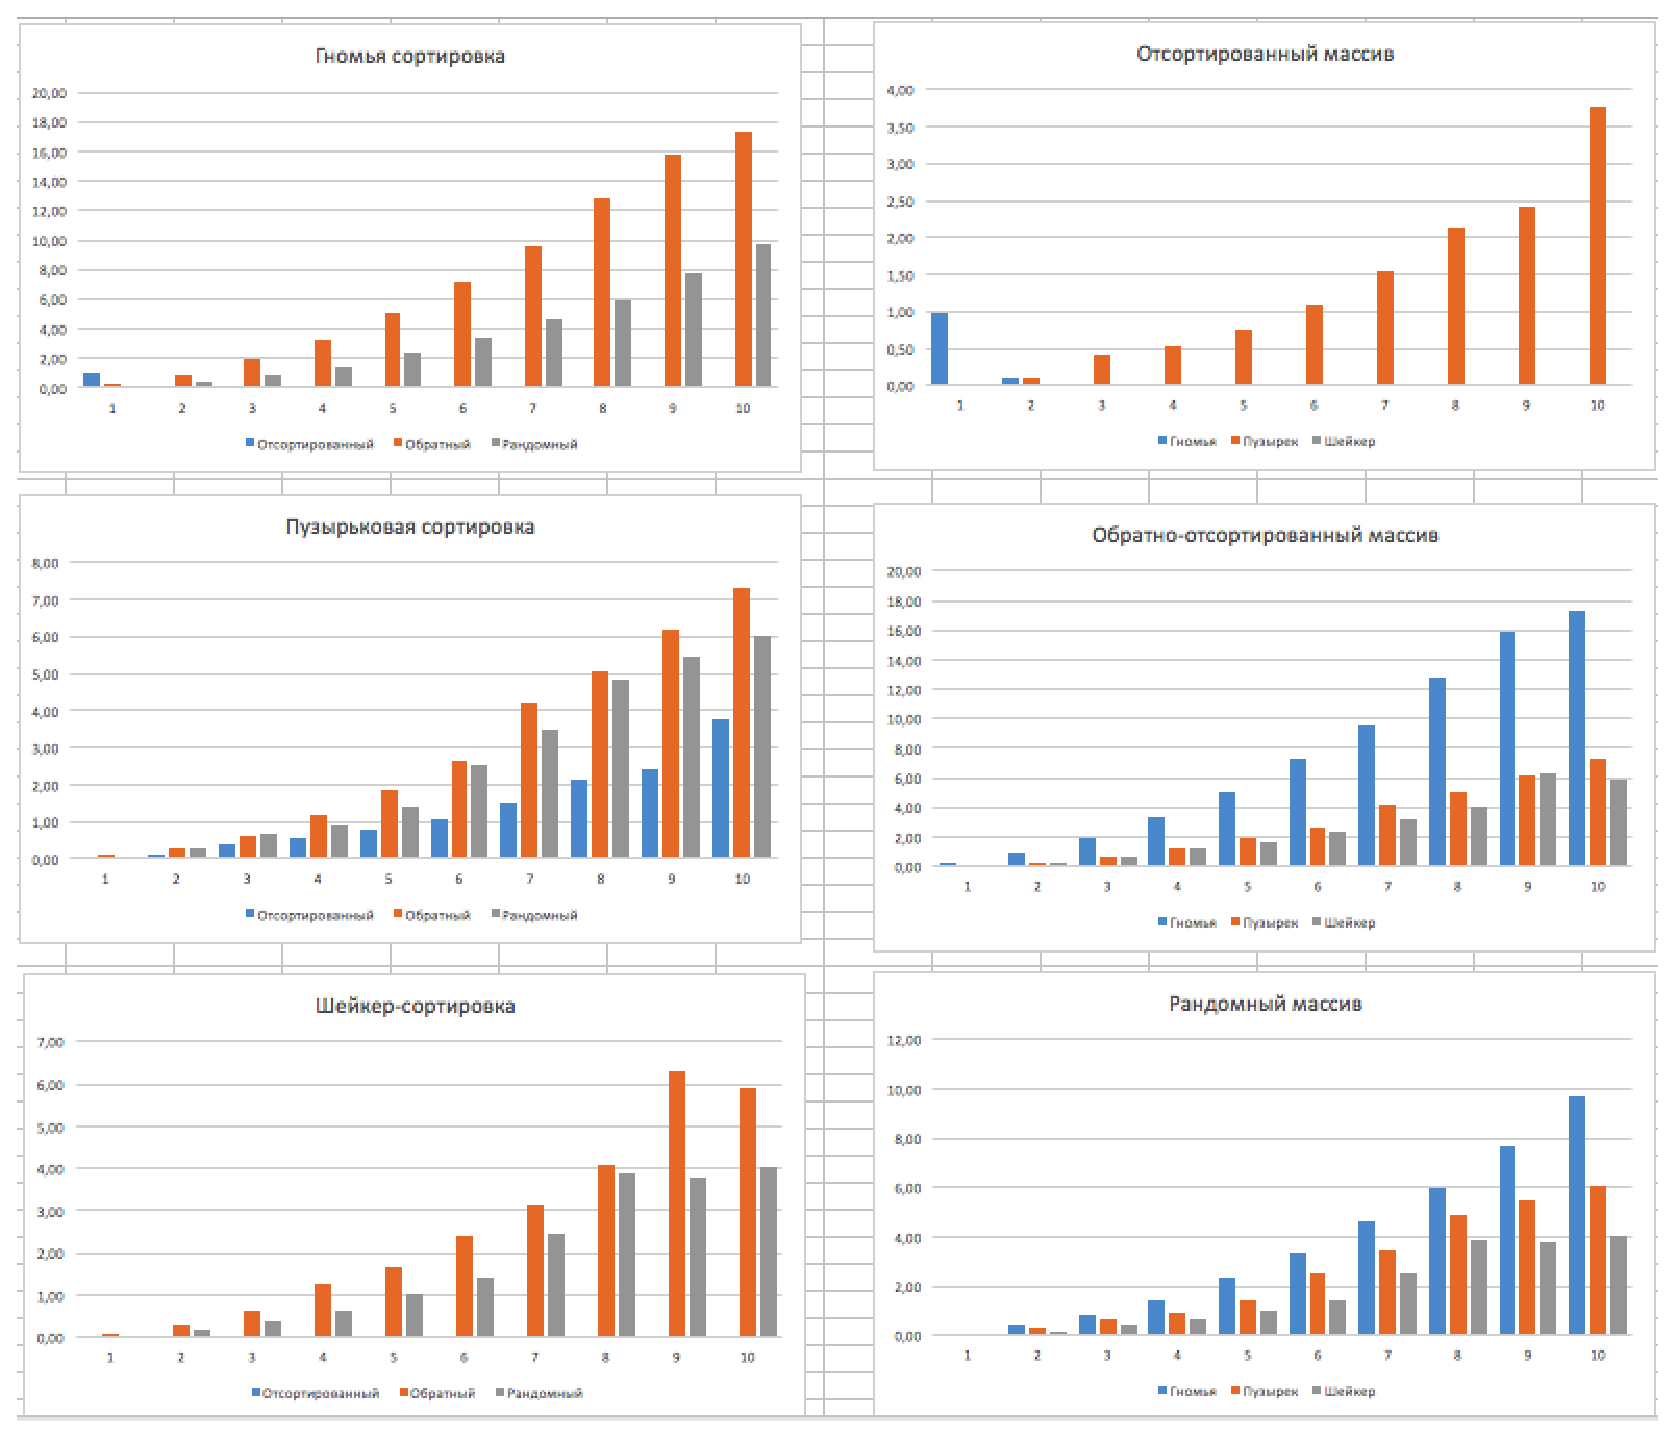
\includegraphics[width=\linewidth]{time}}
		\caption{Сравнение времени при нечетном кол-ве элементов}
	\end{minipage}
\end{figure}

%%%%%%%%%%%%%%%%%%%%%%%%%%%%%%		
\center{\section{Модель вычислений}}
\flushleft
Операнды +, -, *, /, <, >, <=, >=, ==, !=, [ ] имеют значение f = 1;\\
Значение для цикла f = 2 + N(...), где N - количество итераций.

\newpage
\center{\section{Рассчет сложности алгоритмов}}
\flushleft

\textbf{Гномий алгоритм:}
\begin{enumerate}
	\item Лучший случай(отсортированный массив) : $ \sim O(n)$
	\item Худший случай(отсортированный обратно) : $\sim O(n^2)$
\end{enumerate}	

\textbf{Пузырьковый алгоритм:}
\begin{enumerate}
	\item Лучший случай(отсортированный массив) : $2+n*(2+2+n*(2+3)) = 5*n^2 + 4*n + 2 \sim O(n^2)$
	\item Худший случай(отсортированный обратно) : $2+n*(2+2+n*(2+10)) = 12*n^2 + 4*n + 2 \sim O(n^2)$
\end{enumerate}	

\textbf{Алгоритм шейкера:}
\begin{enumerate}
	\item Лучший случай(отсортированный массив) : $\sim O(n)$
	\item Худший случай(отсортированный обратно) : $\sim O(n^2)$
\end{enumerate}		



%%%%%%%%%%%%%%%%%%%%%%%%%%%%%%		

\newpage
\center{\section{Выводы}}


В результате проведенных испытаний алгоритмов было установлено, что:
\begin{enumerate}
	\item Алгоритм Шейкера значительно быстрее пузырька и гномьей сортировки, особенно на отсортированном наборе данных.
	\item Гномий алгоритм самый базовый и медленный из рассмотренных, однако он имеет линейную сложность при наилучшем случае
	\item У пузырька и в худшем, и в лучшем случае квадратичная сложность, что делает его "усредненным" алгоритмом по времени и сложности среди приведенных
\end{enumerate}

%%%%%%%%%%%%%%%%%%%%%%%%%%%%%%	

\newpage
\center{\section{Заключение}}


\flushleft
В ходе лабораторной работы были реализованы 3 алгоритма сортировок : гномий, пузырьковый и шейкер. Были получены навыки работы с контейнером std::vector в C++, Работой с паттернами проектирования и ООП, а так же с \LaTeX. Изучен подход к вычислению сложности алгоритмов.